%%%%%%%%%%%%%%%%%%%%%%%%%%%%%%%%%%%%%%%%%%%%%%%%%%%
%
%  New template code for TAMU Theses and Dissertations starting Spring 2021.  
%
%
%  Author: Thesis Office
%  
%  Last Updated: 1/13/2021
%
%%%%%%%%%%%%%%%%%%%%%%%%%%%%%%%%%%%%%%%%%%%%%%%%%%%

%%%%%%%%%%%%%%%%%%%%%%%%%%%%%%%%%%%%%%%%%%%%%%%%%%%%%%%%%%%%%%%%%%%%%%
%%                           SECTION I
%%%%%%%%%%%%%%%%%%%%%%%%%%%%%%%%%%%%%%%%%%%%%%%%%%%%%%%%%%%%%%%%%%%%%


\pagestyle{plain} % No headers, just page numbers
\pagenumbering{arabic} % Arabic numerals
\setcounter{page}{1}


\chapter{\uppercase {Introduction}}
\label{cha:Introduction}
This dissertation introduces information quality research into the electricity market monitoring industry, a regulatory component of organized electric markets in the United States \cite{ferc1}. Organized electric markets are a critical component of the North American Bulk Electric System (BES) and its function to reliably and economically deliver power to consumers. Often touted as the "world's largest machine" \cite{stenvignils} by electrical industry staff, the BES has become important to the lives of virtually every resident of the United States, Canada, and a portion of Mexico.

Given the high volume and value of transactions across multiple energy products, there are abundant incentives for market participants to manipulate these markets. Market monitors are the group of professionals that work to ensure that the electricity markets utilizing the BES remain fair, efficient, and open-access. They ensure this by identifying and referring behavior that violates established marketplace rules to the Federal Energy Regulatory Commission (FERC). Wholesale markets clear billions of dollars (USD) in revenue each year. Figure \ref{fig:price-trend-line} displays overall energy consumption and cost for one of these markets, Southwest Power Pool's (SPP) marketplace, from 2020 to 2023.\footnote{Across the time frame shown in Figure \ref{fig:price-trend-line}, the observed market generated an average revenue of over \$9.5 billion, serving an average energy load of over 261 GWh. This figure was generated using data combined from multiple public reports \cite{spp-asom-2023}, \cite{spp-asom-2022}, \cite{spp-asom-2021}, \cite{spp-asom-2020}.}

\begin{figure}[h]
\centering
\fbox{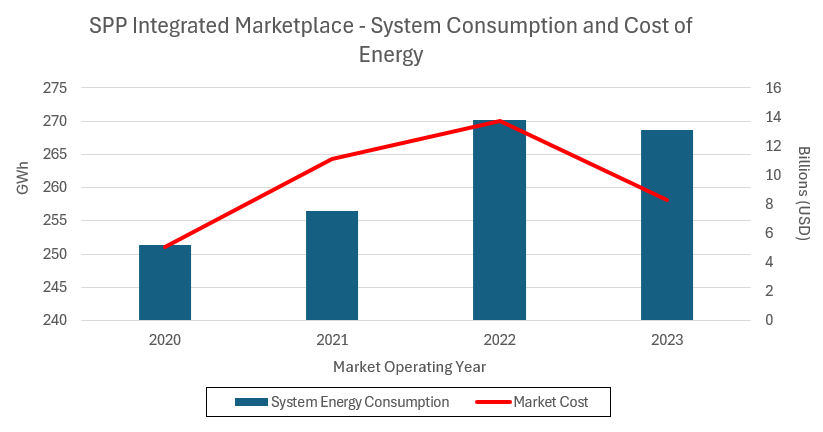
\includegraphics[scale=0.60]{graphic/spp_im_cost.png}}
\caption{Four Year Overall Cost of Energy, SPP Integrated Marketplace}
\label{fig:price-trend-line}
\end{figure}

To illustrate the opportunity that superimposing information quality research onto the market monitoring domain presents, this chapter shall introduce the concepts of the BES, electric markets, and market monitoring, and provide detail as to how applying information quality concepts to market monitoring will help address a previously unsolved problem within the industry.

\section{The North American Bulk Electric System}

The BES\footnote{The North American Electric Reliability Corporation (NERC) serves as the Electric Reliability Operator (ERO) for the BES. In their Glossary of Terms (see References section), the BES refers to all high-voltage transmission lines and substations, generation resources, and all other equipment used in both inter/intra-state transmission of electric capacity.}
is a highly integrated system that facilitates the transmission of electric power (generalized as “energy”) from generation to energy consumption (generalized as a “load”) in a real-time and balanced\footnote{The term “balancing” refers to the need to only generate power as it is needed for consumption, subject to system capacity and economic constraints.}
manner. Built with more than 500,000 miles \cite{nrel1} of physical transmission cabling and over 70,000 electrical substations \cite{cisa-gov}, the BES constantly serves energy to North American consumers and industries alike. With few (relatively recent) exceptions\footnote{Storage resources are a developing technology that can store energy for deployment during reliability emergencies or intervals of energy scarcity.}
, energy is not stored in the system; it is generated (in response to a demand forecast) and then immediately transmitted and consumed by various loads. Figure \ref{fig:BES_1} shows a conceptual configuration of some of the components\footnote{An important distinction to note is between the \textit{utility} and \textit{retail} sectors shown in Figure \ref{fig:BES_1}. While referred to by several names (i.e. wholesale), utility generation and transmission refers to bulk energy (on the scale of MW) that is transmitted on the BES. The retail sector involves distribution of energy to residences and low consumption (on the scale of kW) commercial enterprises. This research focuses on wholesale energy markets, and thus is concerned with the bulk power generation and transmission domains.}
involved in the operation of the BES. \cite{devasia}

\begin{figure}
\centering
\fbox{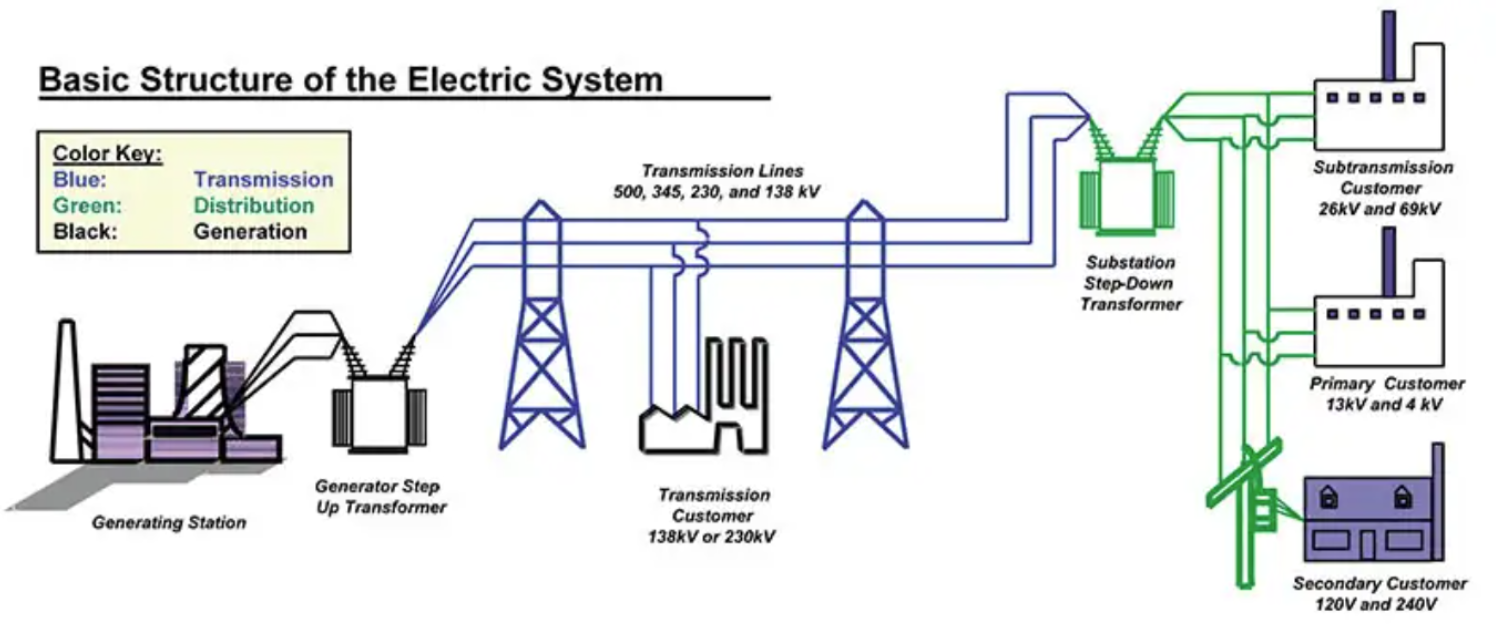
\includegraphics[scale=0.410]{graphic/basic-structure-of-the-bes.png}}
\caption{A Conceptual Illustration of the Bulk Electric System (source: \cite{devasia})} 
\label{fig:BES_1}
\end{figure}

The BES must be precisely managed, at all times, to balance power across the system and to exactly serve the load. Deviations can create instances of voltage and frequency instability that have the potential to significantly damage BES infrastructure. Oftentimes, these deviations are caused by larger environmental events, such as periods of extreme hot or cold weather. Demand for electricity increases during these events\footnote{Notable weather events that have materially impacted BES reliability include the 2020 Californian heat wave, as well as severe winter weather storms in 2021 and 2022 \cite{balancing2}.}, as do generator outages and fuel delivery problems \cite{balancing1}.
No one entity manages the entire BES. Instead, this job is shared across different types of regional entities covering different geographic locales. This dissertation focuses, specifically, on organized markets, which pool resources managed by a Regional Transmission Organization (RTO) or an Independent System Operator (ISO). These entities serve multiple roles; their primary role is to function as grid operators. 

These organizations frequently act as Reliability Coordinators (RC) and Balancing Authorities (BA), monitoring power flows, balancing the grid, and acting to restore system reliability during and after emergencies. They also operate energy markets. Using complex optimization, the RTO/ISO dispatches individual resources in economic order\footnote{\textit{Economic order} refers to the stacking of generator energy offers, in order, from least expensive to most expensive.} while respecting systems constraints, a concept termed security-constrained economic dispatch (SCED)\footnote{Economic dispatch ("ED") is a concept that blends economics and the physical reality of the electric grid.}. It also serves as a revenue-neutral clearing house for the bulk of energy and transmission-related transactions (as well as various financial products).

Serving these various functions to provide electricity generates enormous amounts of data on an hourly basis. This data is widely diverse in terms of sourcing, formatting, usage, sensitivity, and volume. It is the data assets generated by the operation of the BES that serve as the focus of this dissertation, specifically the data generated by \textit{electricity markets}.

\section{An Introduction to Electricity Markets}

As stated above, this research focuses on organized markets. A large portion of the BES includes centrally organized electricity markets. Electricity markets are of great importance to all stakeholders involved in the BES; they allow energy to be economically generated and purchased at the wholesale level.

\begin{figure}[ht]
\centering
\fbox{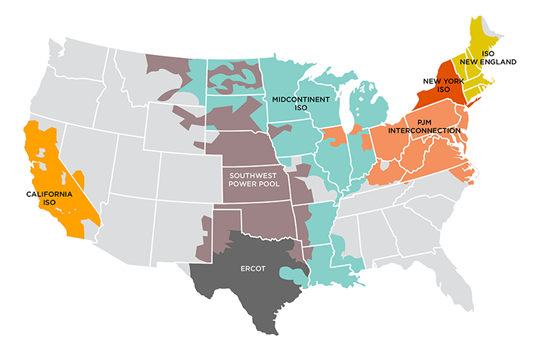
\includegraphics[scale=0.95]{graphic/iso_rto_map.png}}
\caption{Prevailing Energy Market Territories (source: \cite{ferc1})}
\label{fig:gridmap}
\end{figure}

Figure \ref{fig:gridmap} displays, at a high level, how the US energy grid is divided into different territories and notes the name of the entity that runs the organized market. These territories are typically governed by FERC, with the exception of Texas\footnote{ERCOT, the electric system operator for Texas, is not within the jurisdiction of FERC. The Public Utility Commission of Texas, instead, has oversight of the ERCOT market territory. Alaska and Hawaii, additionally, maintain isolated electricity infrastructures.}.

\subsection{Entities}
Electricity markets are operated by a small number of operational entities\footnote{The entities referred to in this chapter are not limited to the 2 categories listed. They also include Transmission Owners and Operators (TOs / TOPs), Regional Entities (REs), Balancing Authorities (BAs), Reliability Coordinators (RCs), and Federal Power Agencies. Oftentimes, an RTO or ISO will also support one or more of these functions (SPP, for example, hosts operational desks for performing reliability coordination).}
within North America. These entities mostly fall under the jurisdiction of FERC (see Figure \ref{fig:gridmap}). The prominent entities that are impacted by market monitoring include Independent System Operators (ISO) and Regional Transmission Organizations (RTO). These entities are filed as non-profit businesses and typically perform similar functions. FERC Orders 888 and 889 initiated the formalized incorporation of an ISO, while FERC Order 2000 set forth the criteria that differentiate an ISO from an RTO.

\subsubsection{Independent System Operator (ISO)}

ISOs are organizations that manage power generation and transmission across the bulk electric system. They operate in an advisory capacity for generation owners (public and investor owned utilities, as well as independent power producers) and transmission owners and operators to effectively generate and trade power in an energy market. A common, helpful analogy that describes the function of an ISO is an air-traffic controller.

Air-traffic controllers merely monitor and route airplane traffic across the airspace over the United States. They own neither physical airplanes nor airlines, and function only as advisors to ensure safe passage of both private and commercial airplanes. ISOs work in a similar fashion. The ISO over the California energy market territory (CAISO) owns none of the transmission infrastructure across which electric power is shipped. However, CAISO manages the flow of energy across this system, and sends regular dispatch instructions to the generators that inject power into the BES.

\subsubsection{Regional Transmission Organization (RTO)}

RTOs are another entity that manage organized markets. They are categorized by a group of four core characteristics (and an additional seven broad operational functions) that separate them from independent system operators. RTOs and ISOs share many similarities. Their operations are regulated by the same government entities, namely FERC and NERC, and they both have the same, conceptual goal: to reliably generate and deliver energy at competitive rates. 

Both entities influence and deploy energy products and maintain both the configuration of their operating territory as well as the flow of energy across the BES. They also both support development and maintenance of open access transmission tariffs (OATT) that allow for unprejudicial access to energy under US federal law. And, most relevant to this research, they are both required to employ a market monitoring group to screen their organized markets for cases of market manipulation.

Their differences primarily lie in how their corporate structures are filed. Both types of entities must be registered non-profit organizations. However, ISOs have more flexibility where impartiality is concerned. RTOs work to maintain independence from their market participants and strictly focus on system reliability and economic efficiency. While ISOs are also concerned with these goals, they have the ability to lobby government on behalf of their members.

\subsection{Types of Markets}

Electricity markets are designed to serve one of several purposes. ISOs typically deploy and operate these different market designs, in concert, as a \textit{marketplace} \cite{ferc2}. Southwest Power Pool's (SPP) Integrated Marketplace is such an example of this. To understand the scope of market monitoring activities, it is important to understand the main energy market designs that exist today. Arguably, there are five main types of electric energy market designs; each design may be deployed with possible variations on its theme (a marketplace that does not operate the function of a capacity market is one such example). Reference Table \ref{tab:mktdesign} for information on prevailing design types.

\begin{table}[ht]
    \centering
    \renewcommand{\arraystretch}{1.2} % Adjust row height
    \begin{tabular}{|p{4.5cm}|p{11cm}|}  % Set fixed column widths
        \hline
        \textbf{Market Type} & \textbf{Purpose} \\ 
        \hline
        Capacity & Allows a load to purchase an agreement of firm capacity for service in the future, usually on the scale of months to years in the future. \\ 
        \hline
        Day-Ahead (DA) & Allows buyers and sellers to secure positions a day before the market sells energy to be consumed (operating day). This aids in realistic price formation. \\ 
        \hline
        Real-Time (RT) & Allows for adjustments between the DA market (what was expected on the day prior) and the system conditions that happen on the operating day. \\ 
        \hline
        Ancillary Services (AS) & Allows other providers to sell products that support grid reliability. For example, the ability of a generator to quickly “ramp up” to a certain production requirement is such a product sold in an AS market. \\
        \hline
        Transmission Congestion \newline Rights (TCR) & Allows participants to hedge against congestion on the transmission system (adequate power can be produced in an area, but there may be difficulties in transmitting it to where it is consumed). \\
        \hline
    \end{tabular}
    \caption{Prevailing Electricity Market Designs}
    \label{tab:mktdesign}
\end{table}

\subsection{BES Complexity and Energy Markets}

The BES is a physical system upon which we superimpose a conceptual, economic market. This dichotomy is part of what makes the energy market so complex to both understand and govern with the data that it generates. Physical machines require continuous diagnostics to ensure that they are operating 1) effectively and 2) within adequate maintenance tolerances. The BES is no different.

Thermal generators that produce electricity are monitored for metrics including: wattage output, fuel consumption, and greenhouse gas emissions. High-voltage transmission lines are monitored for temperature (heat is generated via electricity loss across conductors) and short-circuit events. Substations are monitored for transformer faults, tap configurations, and other mechanical system measurements. Each of these values is typically transmitted in a time-series format, resulting in constant streams of monitoring data. These time series data streams are typically parsed into \textit{market intervals} that constitute "units of work" for market activity. Much of the analysis performed on wholesale electricity markets utilizes data secured from market intervals. Depending on the type of market that is under observation, an interval may range from a span of several seconds (dispatch instructions) to "between five and fifteen minutes" \cite{ferc1} (for calculation of real-time market prices). 

These diagnostic data are only a fraction of the data that are used in the operation of the BES, and much of it feeds into market systems\footnote{While market systems are composed of many different products, they are generally referred to as a \textit{market clearing engine}.} to calculate a realistic price of power at different locations throughout a market territory. Once the market solves, and locational prices are calculated, the market then must be \textit{settled}\footnote{Settlements are also facilitated by shadow accounting, a process of maintaining a separate system (in addition to a production accounting system) to track transactions and ensure that accounts are appropriately balanced.}. Market settlements are another area of market operations that generates complex and voluminous data. In SPP's Integrated Marketplace, the Marketplace Protocols set forth an extensive settlement plan that determines how charges and credits are calculated and assigned to market participants. These settlement instructions also cover events where the market must be "repriced", or re-settled, due to external factors that occur during the operation of a market, such as equipment outages, data communication errors\footnote{Data elements used to monitor and dispatch generation in the BES are collected and shared in the form of \textit{SCADA} (Supervisory Control and Data Acquisition) \cite{scada1}.}, or extreme weather events.

\section{What is Market Monitoring?}

Market monitoring is a discipline that sits at the intersection of two major knowledge domains: \textit{forensics} and \textit{economics}. As such, it takes a scientific approach to testing and analyzing transactions that occur within a marketplace. According to a report published by the United States Energy Association (USEA), Market Monitoring is a necessary component of markets "to ensure that market(s) participants cannot exercise market power, collude or engage in any other behavior that could give them a market share, or higher profits" \cite{imm-usea}. This need places the authority to request and analyze records generated by the operation of electricity markets into the hands of market monitoring units (MMUs).

Market monitors will generally screen for MP behavior that matches the following criteria:

\begin{itemize}
    \item{Exercised (or attempted to exercise) positions of market power}
    \item{Market gaming through oversights in current market protocols or policy (usually outlined in a governing document, known as a tariff}
    \item{Committed cases of market manipulation through acts of collusion, cross-product manipulation, malevolent influence on price formation, or untoward manipulation schemes (economic withholding, uneconomic production, wash trades, "pump and dump" schemes, etc.)}
\end{itemize}


\subsection{The Fall of Enron Corporation}

The Enron Corporation, a former American-based commodities and energy broker, is a well-known case study in American corporate governance (or, rather, lack thereof). The fall of Enron (first signaled in late 2000) uncovered deep, systemic problems of fraud and deceptive business practices that directly influenced both the market monitoring and information quality (IQ) disciplines. Outwardly, Enron appeared to be a stable and innovative company. At the turn of the century, Enron's books reflected an ownership of \$60 billion in assets. This included an internet-based energy trading desk ("Enron Online") that cleared \$2.5 billion in \textit{daily} energy transactions \cite{enron-financials}. In reality, Enron management operated under a culture of willful non-compliance, including (but not limited to):

\begin{itemize}
    \item{Energy withholding practices that sometimes caused enormous electricity prices in the California wholesale energy market}
    \item{Artificial energy shortages causing regular blackouts\footnote{A blackout (an event where power cannot be served) is a breakdown of a portion of grid infrastructure, caused by "an imbalance between power generation and power consumption" \cite{nerc1}.} within the California service territory}
    \item{Scheduling energy transactions to purely cause congestion on California's electric transmission system}
    \item{Accounting fraud (enabled by a creative use of “mark-to-market” based accounting) which allowed Enron to report expected revenues before they were realized}
\end{itemize}

These manipulative schemes had widespread impacts, including: 1) the bankruptcy of one of the largest utility companies in California, Pacific Gas and Electric (PG\&E), 2) rolling blackouts, 3) increased transmission system congestion, and 4) higher than normal electricity bills for California ratepayers.

Enron’s activities constituted both fraud and a behavior known as \textit{market manipulation}; a form of conduct that attempts to willfully circumvent established market rules in pursuit of (usually) large profits. Their usage of market manipulation, especially in California, was a signal to federal regulators that, at the time, there was not enough oversight in the operation of electricity markets. As a result, the United States Congress passed the Energy Policy Act of 2005 to introduce more stringent regulation over the energy industry.

Enron’s downfall resulted in a near-complete devaluation of their stock\footnote{As Enron entered into legal proceedings, their stock fell to under \$1 per share (from a peak as high as \$90 per share in mid-2000) \cite{enron-stock-chart}. }, the dismantling of Arthur Andersen (the auditor assigned to ensure that Enron was operating within the confines of financial reporting law), and a slew of legislation\footnote{18 CFR § 1c.2 (Prohibition of Electric Energy Market Manipulation) is an example of legislation that places monitoring authority in the hands of MMUs \cite{ecfr1}.} 
serving as the impetus for energy market monitoring in the United States. Additionally, Enron’s scandal was a significant contributor to the passing of the Sarbanes-Oxley (SOX) Act of 2002, imposing strict and detailed requirements on data that is used as input for financial reporting. As a result, SOX became another driving force in the implementation of information quality as both an academic discipline and as a business function.

In the years following the disbanding of Enron Corporation, FERC has pursued many more instances of deceptive behavior in organized energy markets. Through the employ of market monitors and FERC enforcement staff, manipulation cases can be pursued and penalized before they become even more critical threats. Table \ref{tab:market-manipulation} lists several high profile cases of market manipulation that are distinct from the Enron case \cite{jpmorgan} \cite{greenhat} \cite{vitol}.

\begin{table}[ht]
    \centering
    \begin{tabular}{|p{2.5cm}|p{2cm}|p{9cm}|}
        \hline
        \textbf{MP} & \textbf{Damages} & \textbf{Incident} \\
        \hline
		JP Morgan  \newline (2013) & \$410 mm & Purchased and operated antiquated generation plants and offered them in the market as competitive generators \\
		\hline
		GreenHat \newline Energy, LLC \newline (2021) & >\$229 mm & Participated in insider trading to purchase enormous positions in PJM's congestion market \\
		\hline
        Vitol Group \newline (2024) & \$2.3mm & Sold physical power at a loss in the DA market to favor their transmission congestion positions \\
		\hline
    \end{tabular}
    \caption{Prominent Cases of Market Manipulation}
    \label{tab:market-manipulation}
\end{table}


\subsection{Skills of a Market Monitor}

Market monitors are one of several groups that function as "unsung heroes" in electricity markets (and within the larger context of the North American bulk electric system). The work that they perform on a routine basis helps to ensure a reliable and economically sound marketplace for buying and selling energy and energy-adjacent ancillary services. 
Market monitoring units are typically staffed with analysts from a wide variety of both technical and non-technical backgrounds. These include: data analysts, statisticians, economists, accountants, technical writers, engineers, and other corporate staff dedicated to investigating events that occur in their jurisdictional markets.

\begin{figure}[h]
\centering
\fbox{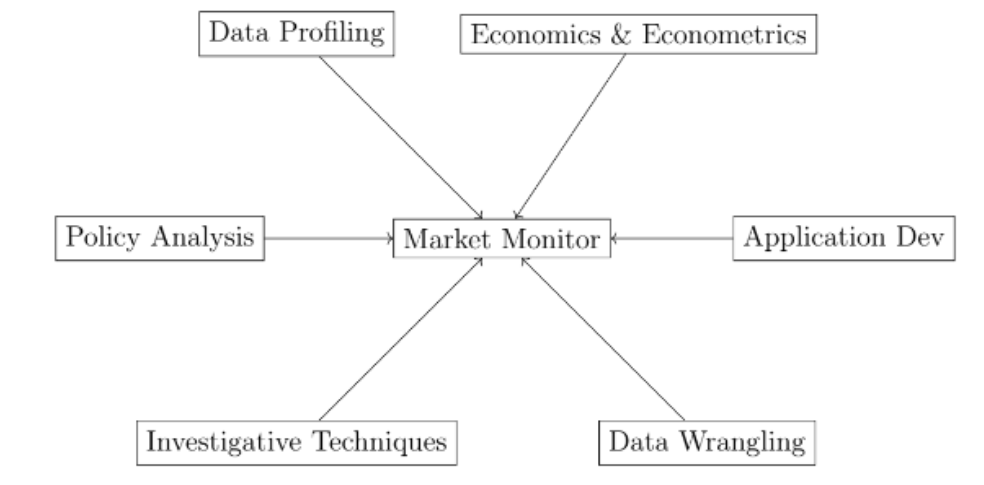
\includegraphics[scale=0.85]{graphic/mkt-monitoring-skill-sets.png}}
\caption{Diverse Skill Sets of a Market Monitor}
\label{fig:skillset}
\end{figure}

Figure \ref{fig:skillset} illustrates a cross-section of several of the skill sets that market monitoring analysts might possess, based on the researcher's experience of working as a market monitor within Southwest Power Pool's (SPP) MMU. As one may imagine, it can be difficult to find an individual contributor that possesses an all-encompassing understanding of each of these knowledge areas.

Market monitors have a wide breadth of responsibilities that must be covered by their individual skill sets. Routine market surveillance is a continuous process that must evolve with the behaviors and trading patterns of market participants. As such, market monitors observe and investigate market bids and offers made each operating day, analyze generator behavior to identify erratic response to dispatch commands, ensure that participants are not covertly colluding or engaging in price fixing\footnote{Energy market prices are typically set on a marginal, spatial basis (representing the cost of injecting another MW of energy, at a location, in a market territory) \cite{lmpfaq}.}, review out-of-market transactions that take place through bilateral settlement schedules (BSS)\footnote{Bilateral settlement schedules are agreements between market participants that are used to trade energy outside of normal market operations \cite{spp-bss}, which help manage credit exposure in the marketplace.}
, and ensure that RTOs and ISOs are acting within the rules defined by their FERC-approved tariff\footnote{A tariff is a governing document that outlines the rules for operating (and participating in) an energy market.} documents (excluding ERCOT, which does not fall under FERC jurisdiction). 

\subsubsection{Market Monitoring Firms}

The current groups involved with electricity market monitoring (both in North America and internationally\footnote{The US Energy Association (USEA) published a report outlining international, independent market monitoring groups. Many of the international groups on this list come from that report (see Appendix \ref{appendix:E}).}) include the organizations compiled in Appendix \ref{appendix:E}. This list is not intended to be exhaustive, as other nations in the Asian-Pacific (APAC), European, and Middle-Eastern (EMEA) regions of the world may not be reflected here. This roster of organizations with market monitoring authority illustrates the number of individuals that are involved with market analysis on an international scale. 

\section{The Case for Information Quality Research in Market Monitoring}

As stated above, market monitoring encompasses a wide range of activities and demands a mix of skill sets. These skill sets must be applied with knowledge learned, over time, from others in the industry. Such activities include gathering transactional market data for screening, calculating metrics for market power\footnote{Market power is often defined as "the ability of a seller to profitably maintain prices above competitive levels for a significant period of time" \cite{rahimi-sheffrin}.}
and concentration analysis (for example, the classic Herfindahl-Hirschman Index [HHI] or the Residual Supply Index [RSI]), mitigating abuses of local market power by market participants, and performing policy analysis to determine efficient market design \cite{goldman} \cite{gao-bompard-napoli-zhou}. 
It also requires calculating known system metrics, Capacity Reserve Margin (CRM) for example\footnote{CRM is a metric (computed by taking the difference between total available capacity and peak system demand) that helps identify "how reliable and prepared the [BES] system has been", in normal operations \cite{jyang}.}, and developing new metrics to measure and track market performance. Data collection, processing, and analysis enables each of these activities, but knowledge on how to make decisions on these data is typically learned through on-the-job training. 

%Data collection, processing, and analysis enables each of these activities, but quality data and the knowledge of how to make %decisions on these data are specialized to the market monitoring domain. This study also highlights a pain point in the current %design of market monitoring units, where the concepts of data confidentiality and maintaining valid performance metrics are %topics of interest that can be difficult to maintain. These directly map to data quality dimensions that IQ-based research can %investigate and improve.

In \textit{Overview of Data Quality: Examining the Dimensions, Antecedents, and Impacts of Data Quality}, one of the antecedents that can directly affect data quality is "information overload" \cite{wang-et-all}. This can be especially true in market monitoring, where users must derive a decision by "fusing" data from many different sources. In instances where users are not familiar with the sources, this has the potential to impact both accuracy and trust in the final product.

As an example in an adjacent industry (utilities), Oyoo's work in data validation for power and utilities organizations showed that information quality can contribute to the development and maintenance of Extract-Transform-Load (ETL) processes \cite{oyoo}. In this example, electric utilities may prioritize data templating and formatting over accuracy and trust. Market monitoring cannot afford to make this trade-off. Market monitors work in complex and high-volume data environments. Systems deployed in these environments must be accessible and user-friendly to help market monitors handle the inherent data and information complexity.

\section{Conducting Information Quality Research in Market Monitoring}

The case study of Enron Corporation sets both a unique and compelling stage for the role that information quality and information science-based research can play in improving the business impact of an independent market monitor. Included amidst Enron Corporation’s numerous failures of governance are a lack of access and an understanding of the complex data generated by the energy industry. The operation of such a large system and marketplace can lead to many siloed data stores, undocumented schemas, and a slew of other information quality-based problems that can also be seen in market monitoring.

Furthermore, the cross-section of skills that market monitors must possess (to effectively perform their job functions) also underscores the importance that data literacy and data quality improvement hold in the market monitoring domain. Both data and system architecture plans, proposed as part of the deliverables of this dissertation, are paramount to designing a system to aid market monitoring staff in their work.

\subsection{Subject Matter Expert (SME) Discussions}

The potential use of this dissertation is driven, in part, by the opinions of subject matter experts in the field of electric energy. In support of this investigation, the researcher has consulted multiple members (in different sectors) of the industry, including two (2) professionals in enterprise asset management, and a separate discussion with a staff member in energy regulation. One such staff member, Kennedy Oyoo, performed information systems research in a different sector of the energy grid, “power and utilities”, focusing on the distribution of electricity to end users.

Energy utilities struggle with a similar issue to those faced by market monitors--- siloed data exists in different systems, and can exist with vastly different data quality scores (in terms of completeness, accuracy, etc.) Oyoo’s research found that a key step, data validation, was missing from the ETL processes of an energy utility. Part of the research completed in his project resulted in an information template-based prototype system that cleansed and validated utility data according to automated assertion rules \cite{oyoo}. Such a methodology has potential impacts for the market monitoring discipline, and may have an influence on the resulting system architecture of this dissertation.

\section{Design Science Methodology}

The roadmap of this project is based on the Design Science Research Methodology (DSRM), a research process for developing new product artifacts. The researcher chose DSRM for this project because the main research objective is to design and develop a domain-specific language for market monitors to use in their analysis.

Data and information quality problems exist today in the market monitoring body of knowledge that a DSL-based system can help address: 

\begin{enumerate}
    \item {Analysts in different teams that arrive at different values when trying to quantify metrics (market impact, for example)}
    \item {Lack of robust metadata assets such as data dictionaries and well-defined data stewardship roles}
    \item {Lack of a mature change management program for software (which, in turn, can impact report reproducibility) }
    \item {A lack of full automation and meta-automation, causing analysts to spend time performing tedious ETL and archival tasks}
\end{enumerate}

Domain-specific languages are powerful models for allowing users to systematically solve problems within a specific domain. As is discussed in the literature review (see Chapter \ref{cha:literature-review}), DSLs have only had limited exposure in electricity markets (and even less exposure in market monitoring). This discovered gap in existing research, complemented by the DQ and IQ issues discussed in the review, serves as the inspiration for this project. Figure \ref{fig:dsrm} provides more detail on the planned use of design science within this project\footnote{See Appendix \ref{appendix:C} for a schedule of the milestones and expected completion timeline for this project.}.

\begin{figure}[h]
\centering
\fbox{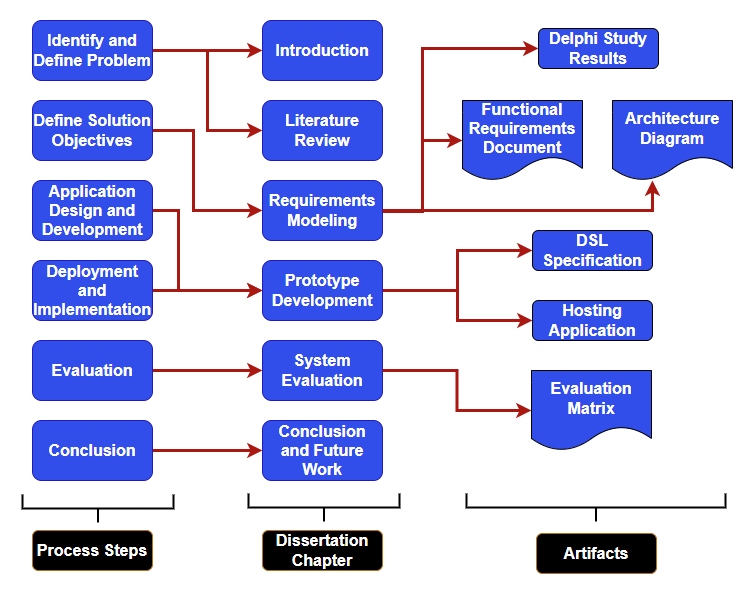
\includegraphics[scale=0.65]{graphic/dsrm_updated_20250819.png}}
\caption{Design Science Research Methodology for this Dissertation}
\label{fig:dsrm}
\end{figure}

\subsection{Proposed Investigation}

In \textit{What Design Science Is Not (2008)}, Baskerville states that one view of design science is to be \textit{generative}. That is, design science leads to the generation of artifacts that then influence the formulation of a theory \cite{design-science-is-not}. This prospect of generativity seems to indicate that a design can be updated based upon empirical evidence. Due to this idea, the researcher chose to employ a Delphi study (as the methodology for gathering expert sentiment) to influence the design of the DSL prototype discussed in this dissertation. The requirements modeling chapter shall discuss the setup, conduct, and results of a Delphi study employed in market monitoring. It then explains how the results of this study influenced the design and requirements document for the prototype system.

Overall, the investigation methodology for this dissertation is composed of five (5) main components. These components include 1) a literature review, 2) a Delphi study to gather opinion and synthesize system requirements, 3) a system architecture design, 4) development of the prototype system (and associated tooling and documentation), and 5) an evaluation discussion to determine to what degree the resultant software satisfies the system requirements.

\subsection{Limitations of this Research}

The scope of work proposed in this dissertation is limited to the objectives outlined in the Proposed Investigation section. Specifically, it shall ultimately evaluate how well the developed prototype functions as a \textit{minimal viable product} (MVP) for energy market analysis.

The proof-of-concept prototype discussed in this dissertation \textbf{is not intended to be a production-ready system}. It is also not expected to be used in a live scenario for market monitors to immediately put into service in support of decision making. The data ingested into the prototype will be based on realistic data scraped from public data systems shown in Appendix \ref{appendix:D}. The evaluation of this system will be based on a matrix (mapping back to the functional requirements document) that "scores" how well the functionality of the prototype supports the intended requirements.

Further system optimization, bug fixes, scalability concerns, and use in live market monitoring scenarios are all currently considered "out of scope" for this dissertation and are reserved for future work. The author, however, may pursue future enhancements to this system as separate research endeavors.